% ---
% Capa
% ---
\imprimircapa
% ---

% ---
% Folha de rosto
% (o * indica que haverá a ficha bibliográfica)
% ---
\imprimirfolhaderosto*
% ---

% ---
% Inserir a ficha bibliografica
% ---
% http://ficha.bu.ufsc.br/
%\begin{fichacatalografica}
%	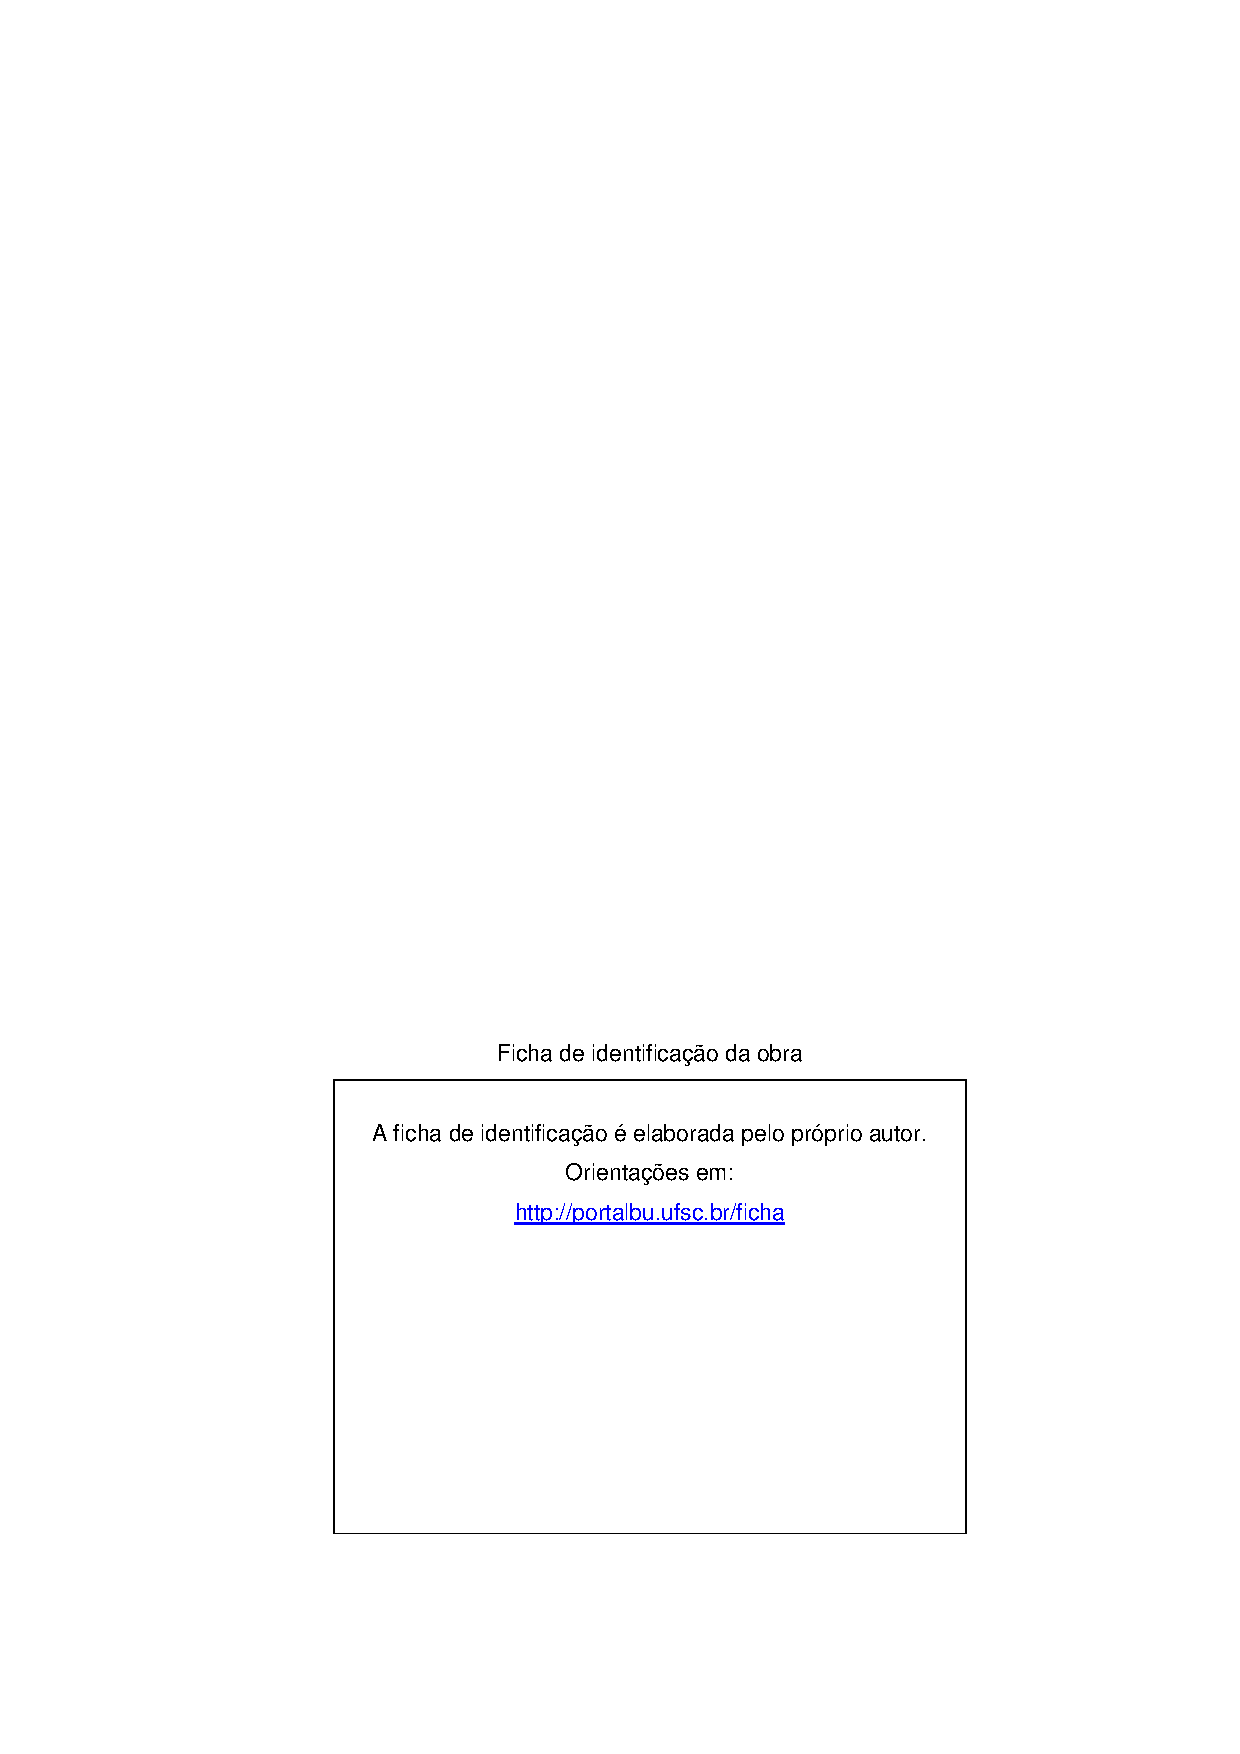
\includepdf{beforetext/Ficha_Catalografica.pdf}
%\end{fichacatalografica}
% ---

% ---
% Inserir folha de aprovação
% ---
%\begin{folhadeaprovacao}
%	\OnehalfSpacing
%	\centering
%	\imprimirautor\\%
%	\vspace*{10pt}		
%	\textbf{\imprimirtitulo}%
%	\ifnotempty{\imprimirsubtitulo}{:~\imprimirsubtitulo}\\%
	%		\vspace*{31.5pt}%3\baselineskip
%	\vspace*{\baselineskip}
	%\begin{minipage}{\textwidth}
	% ~do~\imprimirprograma~do~\imprimircentro~da~\imprimirinstituicao~para~a~obtenção~do~título~de~\imprimirformacao.
%	Este~\imprimirtipotrabalho~foi julgado adequado para obtenção do Título de “\imprimirformacao” e aprovado em sua forma final pelo~\imprimirprograma. \\
%		\vspace*{\baselineskip}
%	\imprimirlocal, \imprimirdata. \\
%	\vspace*{2\baselineskip}
%	\assinatura{\OnehalfSpacing\imprimircoordenador \\ \imprimircoordenadorRotulo~do Curso}
%	\vspace*{2\baselineskip}
%	\textbf{Banca Examinadora:} \\
%	\vspace*{\baselineskip}
%	\assinatura{\OnehalfSpacing\imprimirorientador \\ \imprimirorientadorRotulo}
	%\end{minipage}%
%	\vspace*{\baselineskip}
%	\assinatura{Prof.(a) xxxx, Dr(a).\\
%	Avaliador(a) \\
%	Instituição xxxx}

%	\vspace*{\baselineskip}
%	\assinatura{Prof.(a) xxxx, Dr(a).\\
%	Avaliador(a) \\
%	Instituição xxxx}


%\end{folhadeaprovacao}
% ---

% ---
% Dedicatória
% ---
%\begin{dedicatoria}
%	\vspace*{\fill}
%	\noindent
%	\begin{adjustwidth*}{}{5.5cm}     
%		Este trabalho é dedicado aos meus colegas de classe e a%os meus queridos pais.
%	\end{adjustwidth*}
%\end{dedicatoria}
%---

% ---
% Agradecimentos
% ---
%\begin{agradecimentos}
%	Inserir os agradecimentos aos colaboradores à execução do trabalho. 
	
%	Xxxxxxxxxxxxxxxxxxxxxxxxxxxxxxxxxxxxxxxxxxxxxxxxxxxxxxxxxxxxxxxxxxxxxx. 
%\end{agradecimentos}
% ---

% ---
% Epígrafe
% ---
%\begin{epigrafe}
%	\vspace*{\fill}
%	\begin{flushright}
%		\textit{``Texto da Epígrafe.\\
%			Citação relativa ao tema do trabalho.\\
%			É opcional. A epígrafe pode também aparecer\\
%			na abertura de cada seção ou capítulo.\\
%			Deve ser elaborada de acordo com a NBR 10520.''\\
%			(Autor da epígrafe, ano)}
%	\end{flushright}
%\end{epigrafe}
% ---

% ---
% RESUMOS
% ---

% resumo em português
\setlength{\absparsep}{18pt} % ajusta o espaçamento dos parágrafos do resumo
\begin{resumo}
	\SingleSpacing
	As perdas de hortaliças na cadeia de suprimentos são agravadas pelo transporte de frutos fora dos padrões de comercialização, e os sistemas industriais de classificação óptica têm custo elevado para pequenos e médios produtores. Este trabalho desenvolve e avalia uma bancada de visão computacional de baixo custo que classifica tomates-cereja quanto à maturação, à presença de defeitos e ao tamanho. A bancada usa a câmera de um telefone celular em uma caixa escura e um computador pessoal. As imagens passam por balanço de branco e por segmentação com limiar de Otsu sobre o maior canal de cor, e o tamanho é medido com uma escala calibrada por região com tabuleiro de xadrez. A maturação é classificada pela proporção de cores da superfície, com uma tabela de consulta gerada por um perceptron multicamadas treinado com pixels agrupados por k-means no espaço L*a*b*. Os defeitos são detectados por uma rede neural convolucional ResNet-18 ajustada por transferência de aprendizado com um conjunto próprio de 259 fotos de 97 tomates. Uma interface de operação integra as etapas, indica o destino de cada fruto e registra as inspeções. Na validação cruzada por tomate, a rede obteve acurácia balanceada de 93,6\% $\pm$ 1,9\%. Em um conjunto de teste independente, com 22 tomates, a rede obteve sensibilidade de 84,6\%, especificidade de 88,9\% e F1 de 0,88. A maturação foi acertada em 86,4\% dos tomates, resultado concentrado nos frutos maduros, pois os estádios intermediários não foram distinguidos com confiabilidade. O destino final foi correto em 81,8\% dos tomates, com tempo de processamento de cerca de 54 ms por imagem. Na medição de uma moeda, o erro médio absoluto foi de 0,45 mm. Os resultados indicam a viabilidade da abordagem como prova de conceito, limitada pelo pequeno conjunto de teste e pela iluminação da bancada.

	\textbf{Palavras-chave}: Visão computacional. Tomate-cereja. Classificação de frutos. Rede neural convolucional. Tabela de consulta.
\end{resumo}

% resumo em inglês
\begin{resumo}[Abstract]
	\SingleSpacing
	\begin{otherlanguage*}{english}
		Vegetable losses in the supply chain are increased by shipping fruit that does not meet market standards, and industrial optical sorting systems are too expensive for small and medium growers. This work develops and evaluates a low-cost computer vision bench that classifies cherry tomatoes by ripeness, external defects and size. The bench uses a mobile phone camera inside a dark box and a personal computer. Images are white balanced and segmented with Otsu thresholding on the brightest color channel, and size is measured with a region-wise scale calibrated with a chessboard. Ripeness is classified by the proportion of surface colors, using a lookup table generated by a multilayer perceptron trained on pixels clustered with k-means in the L*a*b* space. Defects are detected by a ResNet-18 convolutional neural network fine-tuned by transfer learning on an in-house set of 259 photos of 97 tomatoes. An operator interface integrates all steps, shows the destination of each fruit and logs the inspections. In tomato-wise cross-validation, the network reached a balanced accuracy of 93.6\% $\pm$ 1.9\%. On an independent test set of 22 tomatoes, it reached a sensitivity of 84.6\%, a specificity of 88.9\% and an F1 score of 0.88. Ripeness was correct for 86.4\% of the tomatoes, a result driven by ripe fruit, because intermediate stages were not reliably distinguished. The final destination was correct for 81.8\% of the tomatoes, with a processing time of about 54 ms per image. When measuring a coin, the mean absolute error was 0.45 mm. The results support the approach as a proof of concept, limited by the small test set and by the bench lighting.

		\textbf{Keywords}: Computer vision. Cherry tomato. Fruit grading. Convolutional neural network. Lookup table.
	\end{otherlanguage*}
\end{resumo}

%% resumo em francês 
%\begin{resumo}[Résumé]
% \begin{otherlanguage*}{french}
%    Il s'agit d'un résumé en français.
% 
%   \textbf{Mots-clés}: latex. abntex. publication de textes.
% \end{otherlanguage*}
%\end{resumo}
%
%% resumo em espanhol
%\begin{resumo}[Resumen]
% \begin{otherlanguage*}{spanish}
%   Este es el resumen en español.
%  
%   \textbf{Palabras clave}: latex. abntex. publicación de textos.
% \end{otherlanguage*}
%\end{resumo}
%% ---

{%hidelinks
	\hypersetup{hidelinks}
	% ---
	% inserir lista de ilustrações
	% ---
	\pdfbookmark[0]{\listfigurename}{lof}
	\listoffigures*
	\cleardoublepage
	% ---
	
	% ---
	% inserir lista de quadros
	% ---
	\pdfbookmark[0]{\listofquadrosname}{loq}
	\listofquadros*
	\cleardoublepage
	% ---
	
	% ---
	% inserir lista de tabelas
	% ---
	\pdfbookmark[0]{\listtablename}{lot}
	\listoftables*
	\cleardoublepage
	% ---
	
	% ---
	% inserir lista de abreviaturas e siglas (devem ser declarados no preambulo)
	% ---
	\glsaddall % as siglas e os símbolos não são marcados com \gls no texto; assim todos entram na lista
	\imprimirlistadesiglas
	% ---
	
	% ---
	% inserir lista de símbolos (devem ser declarados no preambulo)
	% ---
	\imprimirlistadesimbolos
	% ---
	
	% ---
	% inserir o sumario
	% ---
	\pdfbookmark[0]{\contentsname}{toc}
	\tableofcontents*
	\cleardoublepage
	
}%hidelinks
% ---